\documentclass[a4paper, final]{article}

\usepackage[russian]{babel}
\usepackage[utf8]{inputenc}
\usepackage[T1,T2A]{fontenc}
\usepackage[14pt]{extsizes}
\usepackage[left=20mm, top=20mm, right=20mm, bottom=20mm, footskip=10mm]{geometry}
\usepackage{ragged2e}
\usepackage{indentfirst}
\usepackage{hyperref}
\usepackage{graphicx}
\usepackage{tikz}
\usetikzlibrary {arrows.meta,bending,positioning}
\usepackage{caption}
\usepackage{xcolor}
\usepackage{subcaption}
\usepackage{multirow}
\usepackage{mathtools}
\usepackage{tabularray}
\usepackage{xcolor}
\usepackage{amssymb}
\usepackage[figurename=Рис.]{caption}


\definecolor{link_color}{HTML}{0000EE}

\hypersetup{
    colorlinks=true, 
    linkcolor=link_color, 
    urlcolor=link_color, 
    citecolor=link_color
}

% Makes possible using vars
\makeatletter

% Document margins correction
\sloppy

\setlength{\tabcolsep}{0pt}
\renewcommand{\arraystretch}{1}

% Replace eng >= <= to rus ones
\renewcommand{\leq}{\leqslant}
\renewcommand{\geq}{\geqslant}
\renewcommand{\epsilon}{\varepsilon}
\renewcommand{\theta}{\vartheta}
\renewcommand{\phi}{\varphi}

% Макросы для векторного рисунка
\newcommand{\circlenode}{node[minimum size=2.2pt, inner sep=0pt, outer sep=0pt, draw, circle, fill=white] {}}
\newcommand\textnode[3]{node[minimum size=0pt, inner sep=0pt, outer sep=0pt, rotate=#2] {\scalebox{#3}{\footnotesize#1}}}
\newcommand\backgroundnode[3]{node[rotate=#3, fill=white, minimum width=#1, minimum height=#2] {}}

\newcommand\hs[1]{\hspace{#1}}
\newcommand\vs[1]{\vspace{#1}}
\newcommand\s[2]{\scalebox{#1}{#2}}

\newcommand\eq{\hs{-.6pt}=\joinrel\hs{-4pt}=\hs{-.6pt}}
\newcommand\eqv{\hs{-1pt}\equiv\joinrel\hs{-4pt}\equiv\hs{-1pt}}
\newcommand\rarrow{\hs{3pt}-\hs{-5pt}\joinrel\xrightarrow{}}
\newcommand\ti{-\joinrel\hs{-4pt}-}


% Remove space around align
\setlength{\abovedisplayskip}{0pt}
\setlength{\belowdisplayskip}{0pt}
\setlength{\abovedisplayshortskip}{0pt}
\setlength{\belowdisplayshortskip}{0pt}

% Set default latex font
\newcommand\Lcs[1]{{\normalfont\ttfamily\textbackslash#1}}

\renewcommand{\figurename}{Рис.}

% Counters 
\setcounter{table}{0}


\begin{document}


%#################################################################################################


{\thispagestyle{empty}
\begin{center}
    \hfill \break
    \hfill \break
    МИНИСТЕРСТВО НАУКИ И ВЫСШЕГО ОБРАЗОВАНИЯ РОССИЙСКОЙ ФЕДЕРАЦИИ\\[5 pt]
    Федеральное государственное автономное образовательное учреждение высшего образования
    «Санкт-Петербургский политехнический университет Петра Великого»\\[10 pt]
    Институт компьютерных наук и кибербезопасности\\[5 pt]
    Направление: 02.03.01 Математика и компьютерные науки\\[30pt]

    {\large Цифровой практикум}\\[5 pt]
    {\large Отчет о выполнении практических работ №1 и №2}\\[10 pt]
    {\LARGE\bf Верстка математических формул в редакторе \LaTeX}
\end{center}

\vspace{110 pt}

\begin{tabular*}{460pt}{@{\extracolsep{\fill}} l r l}
     Студент,\tabularnewline группы 5130201/40002 & \hspace{50pt} \line(1,0){100} \hspace{-50pt} & Семенов И. А.\\
     & \\
     Руководитель,\tabularnewline доцент ВШТИИ & \hspace{50pt} \line(1,0){100} \hspace{-50pt} & Попов C. Г. \\
     & \\
     & \\
     & \\
     & \multicolumn{2}{r}{\guillemotleft \line(1,0){30} \guillemotright \line(1,0){100} \, 2024г.}
     
\end{tabular*} \\

\vfill

\begin{center}
    Санкт-Петербург, 2024
\end{center}
\newpage
}


%#################################################################################################


{
\begin{center}
    {\large\bf Аннотация}
\end{center}

В данном отчёте по проделанной работе приведён анализ выполнения двух  
лабораторных работ по цифровому практикуму. Лабораторные работы заключались  
в повторении и вёрстке двух документов. В результате выполнения работ были  
получены точные (удалось повторить математические формулы, изображения, текст  
и их расположение на листах) копии данных документов в $.pdf$ файлах, а также  
их код в $.tex$ файлах. Во время выполнения этих работ мной были получены навыки  
работы с \LaTeX{}, достаточные для оформления курсовых работ.  

\newpage
}


%#################################################################################################


\tableofcontents
\newpage
    
    
%#################################################################################################


{
\section*{Введение}
\addcontentsline{toc}{section}{Введение}

\TeX \,— это система компьютерной вёрстки, созданная американским профессором информатики Дональдом Кнутом для реализации компьютерной типографии. Она предоставляет инструменты для секционирования документов, работы с перекрёстными ссылками и точной вёрстки текста. Благодаря этим функциям, \TeX \, пользуется популярностью в академической среде, особенно среди математиков и физиков.
\TeX \,— универсальное средство для создания официальных документов. Использование кода для оформления позволяет пользователю сосредоточиться на содержании. Кроме того, такая особенность упрощает совместную работу, когда несколько авторов добавляют свои части в общий документ.

\LaTeX \,— это наиболее широко используемый набор макрорасширений системы \TeX, предназначенный для упрощения подготовки сложных документов. Типографский набор системы \TeX \,обычно оформляется с использованием \LaTeX. Этот пакет автоматизирует множество задач, включая набор текста на нескольких языках, нумерацию разделов и формул, создание перекрёстных ссылок, размещение иллюстраций и таблиц, ведение библиографии и многое другое. Помимо базового набора, существует большое количество пакетов для расширения возможностей \LaTeX.\cite{wayne-uni:What are LaTeX Packages?}

\newpage
}


%#################################################################################################


{
\section{Постановка задачи}
\par Цель: в точности повторить два выданных листа, используя систему компьютерной вестки \LaTeX. \\
\par Задачи.
\begin{enumerate}
    \item Выбрать и установить среду для вёстки документов.
    \item Сверстать точную копию листа №1 с математическими формулами.
    \item Сверстать точную листа №2, включающего в себя текст, математические формулы и два рисунка.
    \item Сделать отчёт по проделанной работе.
\end{enumerate}
\newpage
}


{
\section{Ход выполнения работы}

\subsection{Выбор редактора для вёрстки 1-го и 2-го листов}

Для работы с \LaTeX{} существует множество редакторов: онлайн-редакторы,  
где компиляция происходит на удалённом сервере, редакторы, специально  
предназначенные для вёрстки \LaTeX{}, как, например, TeXstudio, или редакторы,  
специально не предназначенные для вёрстки \LaTeX{}, однако в них за  
счёт сторонних расширений эту вёрстку можно осуществлять, как, например,  
Visual Studio Code.  

Для вёрстки первого листа использовался Visual Studio Code v1.95, так как  
в нём есть широкие возможности для редактирования текста и подсветки синтаксиса.  
Редактор был скачан с этого сайта: \url{https://code.visualstudio.com/}
Объём дистрибутива составил 136 МБ, объём программы — 1,5 ГБ. Была использована  
среда разработки TeX Live. Компиляция осуществлялась на ноутбуке  
с относительно производительным процессором (AMD Ryzen 5 5500U with  
Radeon Graphics @ 2.10 GHz), 16,00 ГБ оперативной памяти, 64-разрядной  
операционной системой. Работа осуществлялась на Linux (Fedora Workstation 40)\footnote{Дистрибутив Linux, предназначенный для персональных компьютеров (\url{https://docs.fedoraproject.org/en-US/releases/f40/})}.  

Вёрстка второго листа осуществлялась в онлайн-редакторе Overleaf, из-за  
возможности использовать браузерное расширение PerfectPixel\footnote{Браузерное расширение, работающее в Google Chrome и Safary (\url{https://chromewebstore.google.com/detail/perfectpixel-by-welldonec/dkaagdgjmgdmbnecmcefdhjekcoceebi}).} для наложения  
исходного изображения на итоговый документ. Был использован браузер  
Google Chrome v130. Работа осуществлялась на Windows.  

\subsection{Изучение структуры проекта}

Для изучения структуры проекта использовалась книга «\LaTeXe\, в примерах»\cite{book}.  
В \LaTeX{} код делится на две части: преамбулу — в ней объявляются все пакеты, которые  
используются в документе, а также тип и формат документа и макроподстановки  
(например, \verb|\newcommand\s[2]{\scalebox{#1}{#2}}|) — и основную часть, заключённую  
между командами \verb|\begin{document}| и \verb|\end{document}|.
В основной части размещаются текст, формулы, рисунки и таблицы.


\subsection{Выбор пакетов}

Выбор пакетов стал непростой задачей, так как существует множество пакетов,  
которые решают одну и ту же проблему. Из-за этой неоднозначности приходилось искать,  
какой из способов будет оптимальным в том или ином случае, а какой способ может привести  
к последующим проблемам. С выбором пакетов мне помогли ответы людей на таких ресурсах,  
как \textit{stackoverflow} (\url{https://stackoverflow.com/})  
и \textit{tex.stackexchange} (\url{https://tex.stackexchange.com/}).  


\subsubsection{Ниже приведены примеры используемых пакетов:}  
\begin{itemize}  
\item \textit{Для управления параметрами страницы}\newline\verb|\usepackage[textwidth=16cm, textheight=24cm]{geometry}|  

\item \textit{Для вставки изображений в документ}\newline\verb|\usepackage{graphicx}|  

\item \textit{Для русской локализации}\newline\verb|\usepackage[russian,english]{babel}|  

\item \textit{Для добавления красивого русского шрифта}\newline\verb|\usepackage[T2C]{fontenc}|  

\item \textit{Для более тонкой работы с таблицами}\newline\verb|\usepackage{tabularx}|  

\item \textit{Для добавления математических символов}\newline\verb|\usepackage{amssymb}|  

\item \textit{Для векторных рисунков}\newline\verb|\usepackage{tikz}|  

\item \textit{Для создания мультистраничных таблиц}\newline\verb|\usepackage{tabularray}|  
\end{itemize}  

\subsection{Выравнивание и позиционирование текста}  

Так как нужно было получить точную копию исходного листа, позиционирование текста  
стало отдельной задачей. Нужно было учесть отступы от краёв документа, между строками,  
словами и абзацами.  

Для того чтобы задать отступы от краёв документа, был использован пакет $geometry$.  
В нём можно задать параметры $left$, $right$, $top$, $bottom$, которые регулируют отступы  
слева, справа, сверху и снизу соответственно. Таким образом, были заданы отступы от краёв  
документа для 1-го и 2-го листов.  

Чтобы задать отступы между строками, словами и абзацами, были использованы команды  
\verb|\hspace{}|, \verb|\vspace{}| и вручную введённые пробелы, такие как: \verb|,|, \verb|;|,  
\verb|\quad|. Также были использованы такие теги, как \verb|\centering| (позволяет центрировать текст на странице).  

\subsection{Вёрстка математических формул}  

Так как \TeX\, создавался во многом для литературы, связанной с математическим языком,  
в нём есть очень продвинутая система вёрстки формул. Существует множество справочников,  
описывающих способы задания формул, включая различные операторы, символы,  
математические структуры и их стили отображения.  

В \TeX\, можно легко комбинировать текст с формулами, а также задавать их в различных  
режимах — от простых алгебраических выражений до сложных интегралов, матриц,  
сумм и пределов. Чтобы понять, как вёрстать формулы в \LaTeX\,, были использованы как  
материалы из книги «\LaTeXe\, в примерах»\cite{book}, так и ответы людей на форумах\cite{stackoverflow:Left align block of equations}
и документация Overleaf\cite{overleaf:mathematical-expressions}.  

Формулы задаются в «математическом режиме», который объявляется с помощью знаков  
\verb|$| или \verb|\[ ... \]|.  
С помощью \verb|$| можно вставлять формулы прямо внутрь строки, например, код формулы  
$x^n + y^n = z^n$ будет выглядеть так: \verb|$x^n + y^n = z^n$|. Тогда как формулы,  
заданные с помощью \verb|\[ ... \]|, выносятся за пределы строки и помещаются в центр:  
\[ x^n + y^n = z^n \]  

Также стоит отметить, что при вёрстке первого файла мне встретились многострочные формулы,  
как, например, эта:  

\resizebox{.9\linewidth}{!}{  
    \begin{minipage}{\linewidth}  
        \begin{align*}  
            \hspace{-5pt} \makebox[0pt][l]{$13.^{7}$} \hspace{5pt} \hspace{23.5pt} \int_{0}^{\pi} \sin^{2n+1}x&\cos2mx \,dx = \\[-2.5pt]  
            & \hspace{5pt} = 2\hspace{-2pt}\int_{0}^{\pi/2} \sin^{2n+1}x\cos2mx \,dx = \frac{(-1)^{m}2^{n+1}n!(2n+1)!!}{(2m-2n-3)!!(2m+2n+1)!!} & \, [n \geq m - 1] \\[-3pt]  
            & \hspace{5pt} = \frac{(-1)^{n+1}2^{n+1}n!(2m-2n+3)!!(2n+1)!!}{(2m+2n+1)!!} & \, [n < m - 1] \\  
            \tag*{ГХ2 (332)(12c) \hspace{-.5pt}}  
        \end{align*}  
    \end{minipage}  
}  

Ниже приведён код этой формулы:  

\begin{small}  
\begin{verbatim}  
1 \begin{align*}  
2    \hspace{-5pt} \makebox[0pt][l]{$13.^{7}$} \hspace{5pt}  
     \hspace{23.5pt} \int_{0}^{\pi} \sin^{2n+1}x&\cos2mx \,dx = \\[-2.5pt]  
3    & \hspace{5pt} = 2\hspace{-2pt}\int_{0}^{\pi/2} \sin^{2n+1}x\cos2mx  
     \,dx = \frac{(-1)^{m}2^{n+1}n!(2n+1)!!}{(2m-2n-3)!!(2m+2n+1)!!}  
     & \, [n \geq m - 1] \\[-3pt]& \hspace{5pt} =  
     \frac{(-1)^{n+1}2^{n+1}n!(2m-2n+3)!!(2n+1)!!}{(2m+2n+1)!!}  
     & \, [n < m - 1] \\  
4    \tag*{ГХ2 (332)(12c) \hspace{-.5pt}}  
5 \end{align*}  
\end{verbatim}  
\end{small}  

Как нетрудно заметить, выравнивание формул в \LaTeX\, можно делать с помощью \verb|\begin{align} ... \end{align}|\cite{overleaf:aligning-equations}.  


\subsection{Создание графических изображений} 
\TeX , позволяет вставлять в документ растровые и векторные изображения, для которых были использованы пакеты $graphicx$ и $TikZ$ соответственно. 

Пакет $graphicx$ позволяет вставлять в документ $png$ изображения. Можно задавать ширину, высоту, увеличение $(scale)$ и другие параметры.

Например, так выглядит код для добавления растровой картинки, вставленной с помощью пакета $graphicx$: 

\begin{small} 
\begin{verbatim} 
\begin{figure}
    \includegraphics{graph.png} % Загрузка изображения graph.png 
    \caption{$y=\sigma(x)$} % Подпись под изображением 
\end{figure} 
\end{verbatim} 
\end{small}

Пакет $TikZ$, в свою очередь, позволяет строить комплексные векторные изображения, состоящие из множества элементов. С помощью него можно строить графики функций, геометрические фигуры, схемы, диаграммы, блок-схемы, иллюстрации процессов, а также оформлять сложные научные и технические чертежи. Пакет предоставляет пользователю гибкий язык разметки для определения и настройки каждой детали изображения: от расположения узлов и соединений до управления цветами, стилями линий и параметрами текста.

Чтобы упростить вёрстку векторного изображения, была использована таблица, описывающая его параметры. Для исходного изображения (Рис. 1) была построена таблица с каждым объектом, его типом, расположением и параметрами (Таблица \ref{tab:obj}). На основе этой таблицы было построено изображение (Рис. 2), которое путём наложения с помощью PixelPerfect было доведено до полного совпадения с оригиналом.


\begin{figure}[h]
    \centering
    \begin{subfigure}{0.45\textwidth}
        \centering
        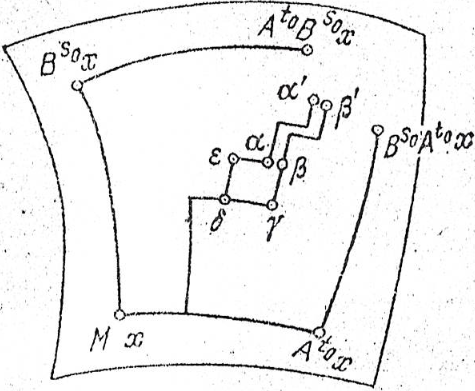
\includegraphics[scale=.64]{./img/rastr-pic.png}
        \caption*{Рис. 1: Оригинал изображения}
        \label{fig:original}
    \end{subfigure}
    \hfill
    \begin{subfigure}{0.45\textwidth}
        \centering
        \begin{tikzpicture}[scale=2.2, transform shape]
            % Внешняя фигура
            \draw [thick]
                (0,0) to[out=168,in=10] 
                (-2.5,.05) to[out=79,in=-60] 
                (-2.86,2.61) to[out=18.5,in=158] 
                (.4,2.7) to[out=-92,in=75] (0,0);
    
            % Внутренняя фигура
            \draw  [thick]
                (.03,1.98) \circlenode to[out=-100,in=70] 
                (-.42,.42) \circlenode to[out=172,in=4] 
                (-1.96,.56) \circlenode to[out=95,in=-65] 
                (-2.29,2.33) \circlenode to[out=25,in=177] 
                (-.51,2.595) \circlenode;

            % Внутренная фигура 2
            \draw [thick]
                (-1.16,1.45) -- 
                (-1.095,1.78) \circlenode  -- 
                (-.83,1.735) \circlenode -- 
                (-.75,2.04) -- 
                (-.52,2) -- 
                (-.48,2.21) \circlenode;

            % Внутренная фигура 3
            \draw [thick]
                (-1.45,.55) to[out=88,in=-90] 
                (-1.42,1.46) to[out=5,in=177] 
                (-1.16,1.45) \circlenode to[out=3,in=170] 
                (-.8,1.39) \circlenode -- 
                (-.71,1.71) \circlenode -- 
                (-.65,1.95) -- 
                (-.43,1.91) -- 
                (-.37,2.17) \circlenode;

            % Текстовые подписи
            \draw 
                (.5,1.9) \backgroundnode{20pt}{7.5pt}{5}
                (.13,1.85) \textnode{$B$}{5}{.7}
                (.25,1.98) \textnode{$s$}{5}{.7}
                (.33,1.91) \textnode{$0$}{-10}{.42}
                (.39,1.88) \textnode{$A$}{5}{.7}
                (.51,1.98) \textnode{$t$}{5}{.6}
                (.59,1.93) \textnode{$0$}{-10}{.42}
                (.7,1.89) \textnode{$x$}{5}{.7}
                
                (-.55,.28) \textnode{$A$}{-22}{.6}
                (-.4,.32) \textnode{$t$}{-22}{.7}
                (-.34,.24) \textnode{0}{-32}{.4}
                (-.24,.18) \textnode{$x$}{-22}{.7}

                (-2.13,.36) \textnode{\textit{M}}{0}{.7}
                (-1.85,.36) \textnode{$x$}{0}{.7}

                (-2.55,2.49) \textnode{$B$}{0}{.7}
                (-2.39,2.62) \textnode{$s$}{0}{.72}
                (-2.3,2.55) \textnode{$0$}{-10}{.4}
                (-2.2,2.5) \textnode{$x$}{10}{.7}

                (-.83,2.8) \textnode{$A$}{-10}{.7}
                (-.68,2.88) \textnode{$t$}{-10}{.65}
                (-.62,2.81) \textnode{$0$}{-20}{.42}
                (-.53,2.75) \textnode{$B$}{-15}{.7}
                (-.35,2.85) \textnode{$s$}{-15}{.7}
                (-.28,2.78) \textnode{$0$}{-30}{.42}
                (-.2,2.70) \textnode{$x$}{-15}{.7}

                (-.2,2.14) \textnode{$\beta'$}{0}{.7}
                (-.58,1.65) \textnode{$\beta$}{0}{.7}
                (-.8,1.23) \textnode{$\gamma$}{0}{.8}
                (-1.21,1.29) \textnode{$\delta$}{0}{.7}
                (-1.22,1.78) \textnode{$\epsilon$}{0}{.7}
                (-.92,1.9) \textnode{$\alpha$}{0}{.7}
                (-.63,2.33) \textnode{$\alpha'$}{0}{.7};
        \end{tikzpicture}
        \caption*{Рис. 2: Полученное изображение}
        \label{fig:result}
    \end{subfigure}
    \label{fig:сколько_убито}
\end{figure}
\centering
\begin{longtblr}[
  caption = {Объекты, использованные для векторного изображения},
  label = {tab:obj},
]{
  colspec = {|c|m{280pt}|c|},
  rowhead = 1
} 
    \hline
    Тип объекта & \centeringПримерные координаты & Параметры \\
    \hline
    Кривая & \begin{tabular}{l}(0,0) $\xrightarrow[\text{in=10}]{\text{out=168}}$ (-2.5,.05) $\xrightarrow[\text{in=-60}]{\text{out=79}}$ \\ $\rightarrow$ (-2.86,2.61) $\xrightarrow[\text{in=158}]{\text{out=18.5}}$ (.4,2.7) $\xrightarrow[\text{in=75}]{\text{out=-92}}$ (0,0) \end{tabular}   & тонкая \\
    \hline
    Кривая & \begin{tabular}{l}(.03,1.98) $\xrightarrow[\text{in=70}]{\text{out=-100}}$ (-.42,.42) $\xrightarrow[\text{in=4}]{\text{out=172}}$ \\ $\rightarrow$ (-1.96,.56) $\xrightarrow[\text{in=-65}]{\text{out=95}}$ (-2.29,2.33) $\xrightarrow[\text{in=177}]{\text{out=-25}}$ \\ $\rightarrow$ (-.51,2.595) \end{tabular}   & тонкая \\
    \hline
    Ломаная & \begin{tabular}{l}(-1.16,1.45) $\rightarrow$ (-1.095,1.78) $\rightarrow$ (-.83,1.735) $\rightarrow$\\$\rightarrow$ (-.52,2) $\rightarrow$ (-.48,2.21) \end{tabular}   & тонкая \\
    \hline
    Кривая & \begin{tabular}{l}(-1.45,.55) $\xrightarrow[\text{in=-90}]{\text{out=88}}$ (-1.42,1.46) $\xrightarrow[\text{in=177}]{\text{out=5}}$ \\$\rightarrow$ (-1.16,1.45) $\xrightarrow[\text{in=170}]{\text{out=3}}$ (-.8,1.39) $\rightarrow$ \\ $\rightarrow$ (-.71,1.71)  $\rightarrow$ (-.65,1.95) $\rightarrow$ \\ $\rightarrow$ (-.43,1.91) $\rightarrow$ (-.37,2.17) \end{tabular} & тонкая \\
    \hline
    Текст & \begin{tabular}{l} $B$ в (.13,1.85), $s$ в (.25,1.98), $A$ в (.39,1.88),\\ $x$ в (.7,1.89) \end{tabular} & \begin{tabular}[c]{@{}c@{}}\smallповорот 5°,\\\smallувел. в 0.7 раза \end{tabular}  \\
    \hline
    Текст & \begin{tabular}{l} $0$ в (.33,1.91), $0$ в (.59,1.93) \end{tabular} & \begin{tabular}[c]{@{}c@{}}\smallповорот -10°,\\\smallувел. в 0.42 раза \end{tabular}  \\
    \hline
    Текст & \begin{tabular}{l} $t$ в (.51,1.98)\end{tabular} & \begin{tabular}[c]{@{}c@{}}\smallповорот 5°,\\\smallувел. в 0.6 раза \end{tabular}  \\
    \hline
    Текст & \begin{tabular}{l} $A$ в (-.55,.28)\end{tabular} & \begin{tabular}[c]{@{}c@{}}\smallповорот -22°,\\\smallувел. в 0.6 раза \end{tabular}  \\
    \hline
    Текст & \begin{tabular}{l} $t$ в (-.4,.32), $x$ в (-.24,.18)\end{tabular} & \begin{tabular}[c]{@{}c@{}}\smallповорот -22°,\\\smallувел. в 0.7 раза \end{tabular}  \\
    \hline
    Текст & \begin{tabular}{l} $0$ в (-.34,.24)\end{tabular} & \begin{tabular}[c]{@{}c@{}}\smallповорот -32°,\\\smallувел. в 0.4 раза \end{tabular}  \\
    \hline
    Текст & \begin{tabular}{l} $M$ в (-2.13,.36), $x$ в (-1.85,.36), \\$B$ в (-2.55,2.49), $\beta$ в (-.2,2.14), $\beta$ в (-.58,1.65),\\ $\delta$ в (-1.21,1.29),  $\epsilon$ в (-1.22,1.78),\\ $\alpha$ в (-.92,1.9), $\alpha'$ в (-.63,2.33) \end{tabular} & \begin{tabular}[c]{@{}c@{}}\smallповорот 0°,\\\smallувел. в 0.7 раза \end{tabular}  \\
    \hline
    Текст & \begin{tabular}{l} $s$ в (-2.39,2.62)\end{tabular} & \begin{tabular}[c]{@{}c@{}}\smallповорот 0°,\\\smallувел. в 0.72 раза \end{tabular}  \\
    \hline
    Текст & \begin{tabular}{l} $0$ в (-2.3,2.55)\end{tabular} & \begin{tabular}[c]{@{}c@{}}\smallповорот -10°,\\\smallувел. в 0.4 раза \end{tabular}  \\
    \hline
    Текст & \begin{tabular}{l} $t$ в (-.68,2.88)\end{tabular} & \begin{tabular}[c]{@{}c@{}}\smallповорот -10°,\\\smallувел. в 0.65 раза \end{tabular}  \\
    \hline
    Текст & \begin{tabular}{l} $0$ в (-.62,2.81)\end{tabular} & \begin{tabular}[c]{@{}c@{}}\smallповорот -20°,\\\smallувел. в 0.42 раза \end{tabular}  \\
    \hline
    Текст & \begin{tabular}{l} $B$ в (-.53,2.75), $s$ в (-.35,2.85), $x$ в (-.2,2.7)\end{tabular} & \begin{tabular}[c]{@{}c@{}}\smallповорот -15°,\\\smallувел. в 0.7 раза \end{tabular}  \\
    \hline
    Текст & \begin{tabular}{l} $0$ в (-.28,2.78)\end{tabular} & \begin{tabular}[c]{@{}c@{}}\smallповорот -30°,\\\smallувел. в 0.42 раза \end{tabular}  \\
    \hline
    Текст & \begin{tabular}{l} $\gamma$ в (-.8,1.23)\end{tabular} & \begin{tabular}[c]{@{}c@{}}\smallповорот 0°,\\\smallувел. в 0.8 раза \end{tabular}  \\
    \hline
    Узел & \begin{tabular}{l}в (.03,1.98), в(-.42,.42), в (-1.96,.56), \\ в (-2.29,2.33),в (-.51,2.595), в (-1.095,1.78),\\ в (-.83,1.735), в (-.48,2.21), в (-1.16,1.45),\\ в (-.8,1.39), в (-.71,1.71), в (-.37,2.17)\end{tabular} & \begin{tabular}[c]{@{}c@{}}\smallмин. размер 2.2пт,\\\smallзаливка белая,\\\smallкруг \end{tabular}  \\
    \hline
\end{longtblr}

\newpage

\subsubsection{Код для построения векторного изображения:}

\begin{small}
\begin{verbatim}
% Макросы для векторного рисунка
\newcommand{\circlenode}{node[minimum size=2.2pt, inner sep=0pt, 
outer sep=0pt, draw, circle, fill=white] {}}
\newcommand\textnode[3]{node[minimum size=0pt, inner sep=0pt, outer
sep=0pt, rotate=#2] {\scalebox{#3}{\footnotesize#1}}}
\newcommand\backgroundnode[3]{node[rotate=#3, fill=white, minimum 
width=#1, minimum height=#2] {}}


\begin{tikzpicture}[scale=1.35, transform shape]
    % Внешняя фигура
    \draw [thick]
        (0,0) to[out=168,in=10] 
        (-2.5,.05) to[out=79,in=-60] 
        (-2.86,2.61) to[out=18.5,in=158] 
        (.4,2.7) to[out=-92,in=75] (0,0);

    % Внутренняя фигура
    \draw  [thick]
        (.03,1.98) \circlenode to[out=-100,in=70] 
        (-.42,.42) \circlenode to[out=172,in=4] 
        (-1.96,.56) \circlenode to[out=95,in=-65] 
        (-2.29,2.33) \circlenode to[out=25,in=177] 
        (-.51,2.595) \circlenode;

    % Внутренная фигура 2
    \draw [thick]
        (-1.16,1.45) -- 
        (-1.095,1.78) \circlenode  -- 
        (-.83,1.735) \circlenode -- 
        (-.75,2.04) -- 
        (-.52,2) -- 
        (-.48,2.21) \circlenode;

    % Внутренная фигура 3
    \draw [thick]
        (-1.45,.55) to[out=88,in=-90] 
        (-1.42,1.46) to[out=5,in=177] 
        (-1.16,1.45) \circlenode to[out=3,in=170] 
        (-.8,1.39) \circlenode -- 
        (-.71,1.71) \circlenode -- 
        (-.65,1.95) -- 
        (-.43,1.91) -- 
        (-.37,2.17) \circlenode;

    % Текстовые подписи
    \draw 
        (.5,1.9) \backgroundnode{20pt}{7.5pt}{5}
        (.13,1.85) \textnode{$B$}{5}{.7}
        (.25,1.98) \textnode{$s$}{5}{.7}
        (.33,1.91) \textnode{$0$}{-10}{.42}
        (.39,1.88) \textnode{$A$}{5}{.7}
        (.51,1.98) \textnode{$t$}{5}{.6}
        (.59,1.93) \textnode{$0$}{-10}{.42}
        (.7,1.89) \textnode{$x$}{5}{.7}
        
        (-.55,.28) \textnode{$A$}{-22}{.6}
        (-.4,.32) \textnode{$t$}{-22}{.7}
        (-.34,.24) \textnode{0}{-32}{.4}
        (-.24,.18) \textnode{$x$}{-22}{.7}

        (-2.13,.36) \textnode{\textit{M}}{0}{.7}
        (-1.85,.36) \textnode{$x$}{0}{.7}

        (-2.55,2.49) \textnode{$B$}{0}{.7}
        (-2.39,2.62) \textnode{$s$}{0}{.72}
        (-2.3,2.55) \textnode{$0$}{-10}{.4}
        (-2.2,2.5) \textnode{$x$}{10}{.7}

        (-.83,2.8) \textnode{$A$}{-10}{.7}
        (-.68,2.88) \textnode{$t$}{-10}{.65}
        (-.62,2.81) \textnode{$0$}{-20}{.42}
        (-.53,2.75) \textnode{$B$}{-15}{.7}
        (-.35,2.85) \textnode{$s$}{-15}{.7}
        (-.28,2.78) \textnode{$0$}{-30}{.42}
        (-.2,2.70) \textnode{$x$}{-15}{.7}

        (-.2,2.14) \textnode{$\beta'$}{0}{.7}
        (-.58,1.65) \textnode{$\beta$}{0}{.7}
        (-.8,1.23) \textnode{$\gamma$}{0}{.8}
        (-1.21,1.29) \textnode{$\delta$}{0}{.7}
        (-1.22,1.78) \textnode{$\epsilon$}{0}{.7}
        (-.92,1.9) \textnode{$\alpha$}{0}{.7}
        (-.63,2.33) \textnode{$\alpha'$}{0}{.7};
\end{tikzpicture}
\end{verbatim}
\end{small}
\newpage

\section{Возникшие проблемы}
\begin{enumerate}
    \item На первом листе возникла проблема выравнивания формул по левому краю. При использовании \verb|\begin{align} ... \end{align}| формулы были выровнены по центру. Решить эту проблему мне помог ответ на \textit{Stack Overflow}\cite{stackoverflow:Left align block of equations}.
    
    \item На первом листе возникла проблема подключения \textit{sans-serif}\footnote{\textit{sans-serif} — шрифты без засечек.} шрифтов. При подключении стороннего шрифта программа при компиляции выдавала ошибку. Проблема была решена сменой среды с \textit{pdflatex} на \textit{lualatex}. Помог мне решить эту проблему ответ на \textit{Stack Overflow}\cite{stackoverflow:pdflatex missing T2A fonts}.
    
    \item На первом листе возникла проблема изменения размера шрифта колонтитула. Проблема была частично решена с помощью \verb|\relscale{.93}|, однако итоговый размер шрифта колонтитула оказался немного меньше, чем в оригинале.
    
    \item При вёрстке второго листа возникла проблема с масштабом векторного рисунка. Эта проблема была решена с помощью документации\cite{tikz:The TikZ and PGF Packages} пакета \textit{TikZ}. Были использованы параметры \verb|scale=1.35, transform shape|.
    
    \item При вёрстке второго листа возникла проблема с выбором инструмента для создания круглых вершин с белой заливкой и чёрной рамкой криволинейного четырёхугольника. В итоге это было сделано с помощью инструмента пакета \textit{TikZ} — \verb|node|. Решить эту проблему мне помогла документация\cite{tikz:A Petri-Net for Hagen} пакета \textit{TikZ}.
\end{enumerate}

\newpage
}


%#################################################################################################


{
\section*{Заключение}
\addcontentsline{toc}{section}{Заключение}

В итоге получилось 2 листа, достаточно точно повторяющих исходные, — настолько, что расхождения можно считать незначительными.

На вёрстку первого листа в сумме было потрачено около 18 часов. Большая часть из них, конечно, была потрачена на то, чтобы разобраться в документации \LaTeX\, и установить на компьютер среду разработки. Также большая часть времени была потрачена на выравнивание 10 формул, чтобы итоговый лист можно было наложить на исходный. Размер \textit{.tex} файла составил 5,46 КБ, сам файл состоял из 124 строчек кода.

На вёрстку второго листа было потрачено около 13 часов. Большая часть времени ушла на то, чтобы сверстать векторный рисунок: разобраться с документацией пакета \textit{TikZ} и решить проблемы, связанные с вёрсткой векторного рисунка. Также значительная часть времени ушла на выравнивание и позиционирование текста: нужно было в точности повторить исходный лист. В итоге удалось сверстать векторное изображение, вставить 22 формулы как в сам текст, так и отдельно (с новой строки), вставить растровый рисунок. Объём \textit{.tex} файла составил 11,7 КБ, сам файл состоял из 209 строчек кода.


\newpage

\addcontentsline{toc}{section}{Список литературы}
\begin{thebibliography}{}
    \bibitem{book} Книга «\LaTeXe в примерах» - Воронцов К. В.

    \bibitem{wayne-uni:What are LaTeX Packages?} «What are LaTeX Packages?» -- [Электронный ресурс]. 
    \newline URL:\thinspace\url{https://guides.lib.wayne.edu/latex/packages} 
    \newline (Дата обращения: 08.09.2024)

    \bibitem{wiki:boxes} «LaTeX/Boxes» -- [Электронный ресурс]. 
    \newline URL:\thinspace\url{https://en.wikibooks.org/wiki/LaTeX/Boxes} 
    \newline (Дата обращения: 20.09.2024)

    \bibitem{overleaf:mathematical-expressions} «Mathematical expressions» -- [Электронный ресурс]. 
    \newline URL:\thinspace\url{https://www.overleaf.com/learn/latex/Mathematical_expressions} 
    \newline (Дата обращения: 08.09.2024)

    \bibitem{overleaf:aligning-equations} «Aligning equations with amsmath» -- [Электронный ресурс]. 
    \newline URL:\thinspace\url{https://www.overleaf.com/learn/latex/Aligning_equations_with_amsmath} 
    \newline (Дата обращения: 10.09.2024)

    \bibitem{stackoverflow:pdflatex missing T2A fonts} «pdflatex missing T2A fonts?» -- [Электронный ресурс]. 
    \newline URL:\thinspace\url{https://stackoverflow.com/questions/73484468/pdflatex-missing-t2a-fonts} 
    \newline (Дата обращения: 25.09.2024)

    \bibitem{stackoverflow:Left align block of equations} «Left align block of equations» -- [Электронный ресурс]. 
    \newline URL:\thinspace\url{https://stackoverflow.com/questions/2632628/left-align-block-of-equations} 
    \newline (Дата обращения: 12.09.2024)
    
    \bibitem{tikz:The TikZ and PGF Packages} «The TikZ and PGF Packages» -- [Электронный ресурс]. 
    \newline URL:\thinspace\url{https://tikz.dev/} 
    \newline (Дата обращения: 22.10.2024)

    \bibitem{tikz:A Petri-Net for Hagen} «A Petri-Net for Hagen» -- [Электронный ресурс]. 
    \newline URL:\thinspace\url{https://tikz.dev/tutorial-nodes} 
    \newline (Дата обращения: 20.10.2024)
  
\end{thebibliography}

\newpage
}
 
 {
\section*{Приложение А. Работа №1. Страница со списком математических формул}
\addcontentsline{toc}{section}{Приложение А. Работа №1. Страница со списком математических формул}
\subsection*{A.1. Исходный лист}
\addcontentsline{toc}{subsection}{A.1. Исходный лист}
\newpage

\subsection*{A.2. Полученный лист}
\addcontentsline{toc}{subsection}{A.2. Полученный лист}
\newpage

\subsection*{A.3. Код}
\addcontentsline{toc}{subsection}{A.3. Код}

\begin{small}
\begin{verbatim}
1 \%!TEX program = lualatex
2 \\documentclass[9pt,fleqn]{article}
3 \usepackage[textheight=24cm, left=2.5cm, right=2.5cm]{geometry}
4 \usepackage{graphicx}
5 % \usepackage[condensed,math]{iwona}
6 \usepackage[russian,english]{babel}
7 \usepackage[T2C]{fontenc}
8 % \usepackage{cmbright}
9 % \usepackage{unicode-math}
10 % \usepackage{polyglossia}
11 \usepackage[no-math,no-config]{fontspec}
12 \setmainfont{calibri.ttf}
13 \usepackage{tabularx}
14 \usepackage{ragged2e}
15 \usepackage{amsmath}
16 \usepackage{relsize}
17 % \setdefaultlanguage{russian}
18 % For russian controls
19 \usepackage{amssymb}
20 \title{Степени тригонометрических функций и линейных функций}
21 \author{Илья Семенов}
22 \pagenumbering{gobble}
23 \newcommand{\verticalGap}{-24pt}
24 % Makes possible using vars
25 \makeatletter
26 % Document margins correction
27 \sloppy
28 % Add new table column styles
29 \newcolumntype{C}[1]{>{\centering\let\newline\\\arraybackslash
    \hspace{0pt}}m{#1}}
30 \newcolumntype{R}[1]{>{\RaggedLeft\arraybackslash}p{#1}}
31 \setlength{\tabcolsep}{0pt}
32 \renewcommand{\arraystretch}{1}
33 % Replace eng >= <= to rus ones
34 \renewcommand{\leq}{\leqslant}
35 \renewcommand{\geq}{\geqslant}
36 % Remove space around align
37 \setlength{\abovedisplayskip}{0pt}
38 \setlength{\belowdisplayskip}{0pt}
39 \setlength{\abovedisplayshortskip}{0pt}
40 \setlength{\belowdisplayshortskip}{0pt}
41 % Set default latex font
42 \newcommand\Lcs[1]{{\normalfont\ttfamily\textbackslash#1}}
43 \begin{document}
44 \begin{tabularx}{16cm}{m{1.6cm} C{12.8cm} R{1.6cm}}
45 \relscale{.93}3.631 & \relscale{.93}\@title & \relscale{.93}
    \textbf{401}\\[-7pt]
46 \rule{16cm}{.6pt}\\[-9pt]
47 \rule{16cm}{.6pt}\\
48 \end{tabularx}
49 \vspace{4pt}
50 \begin{align*}
51 \hspace{-5pt} \makebox[0pt][l]{$7.$} \hspace{5pt} \hspace{23.5pt} 
    \int_{0}^{\pi} \sin^{n}x\cos(2m+1)x \,dx = 0 \\
52 & \tag*{ГХ2 (332)(12a) \hspace{-.5pt}}
53 \end{align*}
54 \vspace{\verticalGap}
55 \vspace{6pt}
56 \begin{align*}
57 \hspace{-5pt} \makebox[0pt][l]{$8.$} \hspace{5pt} \hspace{23.5pt} 
    \int_{0}^{\pi} \sin^{\nu-1}x\cos ax \,dx = \frac{\pi \cos\frac{a 
    \pi}{2}}{2^{\nu-1}\nu\,\mathrm{B}\left(\dfrac{\nu+a+1}{2},\dfrac{
    \nu-a+1}{2}\right)} \\
58 & \hspace{-6pt} [\mathrm{Re}\,\nu > 0] \tag*{Лб V 121(68)и, Вт 337и 
    \hspace{-.5pt}}
59 \end{align*}
60 \vspace{\verticalGap}
61 \begin{align*}
62 \hspace{-5pt} \makebox[0pt][l]{$9.$} \hspace{5pt} \hspace{23.5pt} 
    \int_{0}^{\pi/2} \cos^{\nu-1}x\cos ax \,dx = \frac{\pi}{2^{\nu}\nu\,
    \mathrm{B}\left(\dfrac{\nu+a+1}{2},\dfrac{\nu-a+1}{2}\right)} \\
63 & \hspace{-5pt} [\mathrm{Re}\,\nu > 0] \tag*{ГХ2 (332)(9c) 
    \hspace{-.5pt}}
64 \end{align*}
65 \vspace{\verticalGap}
66 \begin{align*}
67 \hspace{-5pt} \makebox[0pt][l]{$10.$} \hspace{5pt} \hspace{23.5pt} 
    \int_{0}^{\pi/2} \sin^{\nu-2}x\cos\nu x \,dx = \frac{1}{\nu-1}\sin
    \frac{\nu\pi}{2} \\
68 & \hspace{43pt} [\mathrm{Re}\,\nu > 1] \tag*{ГХ2 (332)(16b), Фх II 
    15 2\hspace{2pt}}
69 \end{align*}
70 \vspace{\verticalGap}
71 \vspace{6pt}
72 \begin{align*}
73 \hspace{-5pt} \makebox[0pt][l]{$11.$} \hspace{5pt} \hspace{23.5pt} 
    \int_{0}^{\pi} \sin^{\nu}x\cos\nu x \,dx = \frac{\pi}{2^{\nu}}\cos
    \frac{\nu\pi}{2} \\
74 & \hspace{1.3cm} [\mathrm{Re}\,\nu > -1] \tag*{Лб V 121(70)и 
    \hspace{-.5pt}}
75 \end{align*}
76 \vspace{\verticalGap}
77 \vspace{6pt}
78 \begin{align*}
79 \hspace{-5pt} \makebox[0pt][l]{$12.$} \hspace{5pt} \hspace{23.5pt} 
    \int_{0}^{\pi} \sin^{2n}x\cos2mx \,dx \hspace{-1pt} & = 
    2\hspace{-1.5pt}\int_{0}^{\pi/2} \sin^{2n}x\cos2mx \,dx = \frac{(-1)
    ^{m}}{2^{2n}}\hspace{-2pt}\begin{pmatrix}
80 2n \\
81 n-m
82 \end{pmatrix} \pi \\
83 & = 0 \quad [n < m] \hspace{48pt} \\
84 \tag*{Би (40)(16), ГХ2 (332)(12b) \hspace{-.5pt}}
85 \end{align*}
86 \vspace{\verticalGap}
87 \vspace{-.5pt}
88 \begin{align*}
89 \hspace{-5pt} \makebox[0pt][l]{$13.^{7}$} \hspace{5pt} \hspace{23.5pt}
    \int_{0}^{\pi} \sin^{2n+1}x&\cos2mx \,dx = \\
90 & \hspace{5pt} = 2\hspace{-2pt}\int_{0}^{\pi/2} \sin^{2n+1}x\cos2mx
    \,dx = \frac{(-1)^{m}2^{n+1}n!(2n+1)!!}{(2m-2n-3)!!(2m+2n+1)!!} \quad
    [n \geq m - 1] \\
91 & \hspace{5pt} = \frac{(-1)^{n+1}2^{n+1}n!(2m-2n+3)!!(2n+1)!!}
    {(2m+2n+1)!!} \quad [n < m - 1] \\
92 \tag*{ГХ2 (332)(12c) \hspace{-.5pt}}
93 \end{align*}
94 \vspace{\verticalGap}
95 \vspace{-3.5pt}
96 \begin{align*}
97 & \hspace{-6pt} \makebox[0pt][l]{$14.$} \hspace{5pt} \hspace{23.5pt}
    \int_{0}^{\pi/2} \cos^{\nu-2}x\sin\nu x \,dx = \frac{1}{\nu - 1} 
    \hspace{2.3cm} \\
98 & [\mathrm{Re}\,\nu > 1] \tag*{ГХ2 (332)(16с), Фх II 152}
99 \end{align*}
100 \vspace{\verticalGap}
101 \vspace{6pt}
102 \begin{align*}
103 \hspace{-6pt} \makebox[0pt][l]{$15.$} \hspace{5pt} \hspace{23.5pt} 
    \int_{0}^{\pi} \cos^{m}x\sin nx \,dx \hspace{-1pt} & = [1-(-1)^{m+n}] 
    \hspace{2pt} \int_{0}^{\pi/2} \cos^{m}x\sin nx \,dx = \\
104 & = [1 - (-1)^{m+n}]\hspace{5pt}\Biggl\{\sum_{k=0}^{r-1} \frac{m!}
    {(m-k)!}\frac{(m+n-2k-2)!!}{(m+n)!!} + s\frac{m!(n - m - 2)!!}{(m + 
    n)!!}\Biggr\} \\
105 \end{align*}
106 \vspace{\verticalGap}
107 \vspace{-16pt}
108 \begin{align*}
109 & \vspace{-2pt} \qquad \; \hspace{1cm} \hspace{3pt} \left[\ 
    \hspace{-2pt}r = \begin{cases}
110 m, & \text{если $m \leq n$} \\
111 n, & \text{если $m \geq n$}
112 \end{cases}, \hspace{12pt} s = \\
113 \begin{cases}
114 2, & \text{если $n - m = 4l + 2 > 0$} \\
115 1, & \text{если $n - m = 2l + 1 > 0$} \\
116 0, & \text{если $n - m = 4l$ или $n - m < 0$}
117 \end{cases}\right]\ \tag*{ГХ2 (332)(13a)}
118 \end{align*}
119 \vspace{\verticalGap}
120 \vspace{8pt}
121 \begin{align*}
122 \hspace{-6pt} \makebox[0pt][l]{$16.$} \hspace{5pt} \hspace{23.5pt} 
    \int_{0}^{\pi/2} \cos^{n}x\sin nx \,dx = \frac{1}{2^{n+1}}\sum_{k=1}^
    {n}\frac{2^{k}}{k} \tag*{Фх II 153}
123 \end{align*}
124 \end{document}
    
\end{verbatim}
\end{small}
\newpage

\section*{Приложение Б. Работа №2. Страница из учебника, описывающая «симплекические многообразия»}
\addcontentsline{toc}{section}{Приложение Б. Работа №2. Страница из учебника, описывающая «симплекические многообразия»}
\subsection*{Б.1. Исходный лист}
\addcontentsline{toc}{subsection}{Б.1. Исходный лист}
\newpage

\subsection*{Б.2. Полученный лист}
\addcontentsline{toc}{subsection}{Б.2. Полученный лист}
\newpage

\subsection*{Б.3. Код}
\addcontentsline{toc}{subsection}{Б.3. Код}

\begin{small}
\begin{verbatim}
1 \documentclass[9pt,a5paper]{article}
2 \special{papersize=148mm,210mm}
3 \usepackage[left=2.2cm, right=1.5cm, top=1.5cm, 
    bottom=1.5cm]{geometry}
4 
5 \usepackage{graphicx}
6 \graphicspath{ {./} }
7 
8 \usepackage[russian,english]{babel}
9 \usepackage[T2C]{fontenc}
10 
11 \usepackage{array}
12 \usepackage{tabularx}
13 \usepackage{ragged2e}
14 \usepackage{amsmath}
15 
16 \usepackage{multirow}
17 
18 % Package for graphs
19 \usepackage{tikz}
20 
21 % Package for letterspacing
22 \usepackage[letterspace=300]{microtype}
23 
24 % \setdefaultlanguage{russian}
25 
26 % For russian controls
27 \usepackage{amssymb}
28 
29 \title{СИМПЛЕКТИЧЕСКИЕ МНОГООБРАЗИЯ}
30 \author{Илья Семенов}
31 
32 \pagenumbering{gobble}
33 
34 % Makes possible using vars
35 \makeatletter
36 
37 % Document margins correction
38 \sloppy
39 
40 % Add new table column styles
41 \newcolumntype{C}[1]{>{\centering\let\newline\\\arraybackslash
    \hspace{0pt}}m{#1}}
42 \newcolumntype{R}[1]{>{\RaggedLeft\arraybackslash}p{#1}}
43 
44 \setlength{\tabcolsep}{0pt}
45 \renewcommand{\arraystretch}{1}
46 
47 % Replace eng >= <= to rus ones
48 \renewcommand{\leq}{\leqslant}
49 \renewcommand{\geq}{\geqslant}
50 \renewcommand{\epsilon}{\varepsilon}
51 \renewcommand{\theta}{\vartheta}
52 \renewcommand{\phi}{\varphi}
53 
54 % Макросы для векторного рисунка
55 \newcommand{\circlenode}{node[minimum size=2.2pt, inner sep=0pt, 
    outer sep=0pt, draw, circle, fill=white] {}}
56 \newcommand\textnode[3]{node[minimum size=0pt, inner sep=0pt, 
    outer sep=0pt, rotate=#2] {\scalebox{#3}{#1}}}
57 \newcommand\backgroundnode[3]{node[rotate=#3, fill=white, 
    minimum width=#1, minimum height=#2] {}}
58 
59 \newcommand\hs[1]{\hspace{#1}}
60 \newcommand\vs[1]{\vspace{#1}}
61 \newcommand\s[2]{\scalebox{#1}{#2}}
62 
63 \newcommand\eq{\hs{-.6pt}=\joinrel\hs{-4pt}=\hs{-.6pt}}
64 \newcommand\eqv{\hs{-1pt}\equiv\joinrel\hs{-4pt}\equiv\hs{-1pt}}
65 \newcommand\rarrow{\hs{3pt}-\hs{-5pt}\joinrel\xrightarrow{}}
66 \newcommand\ti{-\joinrel\hs{-4pt}-}
67 
68 % Remove space around align
69 \setlength{\abovedisplayskip}{0pt}
70 \setlength{\belowdisplayskip}{0pt}
71 \setlength{\abovedisplayshortskip}{0pt}
72 \setlength{\belowdisplayshortskip}{0pt}
73 
74 % Set default latex font
75 \newcommand\Lcs[1]{{\normalfont\ttfamily\textbackslash#1}}
76 
77 \begin{document}
78 \hs{-20pt}
79 \begin{tabularx}{\textwidth}{m{.2\textwidth} C{.6\textwidth} 
    R{.2\textwidth}}
80 \footnotesize180& \s{.69}{\@title} & \s{.69}{[ГЛ.8}\hs{100pt}
81 \end{tabularx}
82 
83 \vs{10pt}
84 
85 \small\textbf{Д. Условие коммутативности потоков.} Пусть $\pmb{A}, 
    \hs{5pt} \pmb{B}$ --- векторные поля \hs{2pt} на \hs{1pt} 
    многообразии \hs{2pt} $M$.
86 
87 \vs{-1pt}
88 
89 \small\textls{Теорема}\hs{-1pt}. \hs{.5pt} \textit{Два потока \hs{1pt} 
    $A^{t}, \hs{2pt} B^{s}$ \hs{1pt} коммутируют \hs{1pt} тогда \hs{1pt} 
    и тогда, \hs{2pt} когда \hs{2pt} скобка \hs{4pt} Пуассона \hs{2pt} 
    соответствующих \hs{1pt} векторных \hs{1pt} полей $\pmb{[A,\hs{8pt} B]}$ 
    \hs{.5pt} равна \hs{.5pt} нулю.}
90 
91 \vs{-1.5pt}
92 
93 \small\textls{Доказательство}\hs{-1pt}.\hs{5pt} Если \hs{7pt} 
    $A^{t} B^{s} \eqv B^{s}A^{t}$, \hs{3pt} то \hs{4pt} по \hs{4pt} 
    лемме \hs{6pt}1 $\pmb{[A, \hs{10pt} B]} \eq 0$.
94 \hs{3pt} Если \hs{2pt} $\pmb{[A,\hs{5pt} B]} = 0$, \hs{2pt} то по 
    \hs{1pt} лемме \hs{.7pt} 1 \hs{0pt} для \hs{1pt} любой \hs{1pt} 
    функции $\phi$ \hs{2pt} в \hs{0pt} любой \hs{1pt} точке \textit{x}
95 \vs{-6pt}
96 \[
97 \phi(A^{t}B^{s}x) \hs{2pt} \text{---} \hs{2pt} \phi(B^{s}A^{t}x) \eq 
    o(s^2+t^2), \quad s \rarrow 0, t \rarrow 0. \vs{-3.5pt}
98 \]
99 Мы \hs{1pt} покажем, \hs{1pt} что отсюда \hs{1pt} вытекает \hs{1pt} 
    $\phi(A^{t}B^{s}x) \eq \phi(B^{s}A^{t}x)$ \hs{1pt} при достаточно 
    \hs{1pt} малых \hs{1pt} $s$ \hs{.2pt} и \hs{0pt} $t$.
100 
101 \vs{5pt}
102 
103 \footnotesize \hs{1pt} Применяя это соотношение к \hs{1pt} локальным 
    координатам $(\phi \eq x_1,\,\dots,\,\phi \eq x_n)$, \vs{-11pt}
104 получим $A^{t}B^{s} \eqv B^{s}A^{t}$.
105 \vs{-2pt}
106 \footnotesize \hs{1pt} Рассомтрим прямоугольник \hs{1pt} $0 \hs{1pt} 
    \leq \hs{1pt} t \hs{1pt} \leq \hs{1pt} t_0$, $0 \leq s \leq s_0$ \hs{.2pt}
    (рис. 170) на плоскости \vs{-1pt}\newline 
107 $(t, \hs{2pt} s)$. \hs{-2pt} Каждому пути, \hs{0pt} ведущему \hs{-3pt} из 
    $(0, \hs{2pt} 0)$ \hs{1pt} в $(t_0, s_0)$ и состоящему \hs{1pt} из конечного 
    \vs{-1pt}\newline
108 числа \hs{.5pt} отрезков координатных направлений, сопоставим 
    произведение преобра- \newline зований \hs{1pt} потоков \hs{1pt}
    $A^{t}$ \hs{1pt} и \hs{.5pt} $B^{s}$. Каждому отрезку $t_1 
    \hs{.5pt}\leq\hs{.5pt} l \hs{.5pt}\leq\hs{.5pt} t_2$ \hs{.5pt}
    сопоставим $A^{t_2-t_1}$,
110 \hs{-18pt}
111 \begin{tabular}{m{5.1cm} c}
112         & \multirow{2}{*}{
113             \begin{tikzpicture}[scale=1.35, transform shape]
114                 % Внешняя фигура
115                 \draw 
116                     (0,0) to[out=168,in=10] 
117                     (-2.5,.05) to[out=79,in=-60] 
118                     (-2.86,2.61) to[out=18.5,in=158] 
119                     (.4,2.7) to[out=-92,in=75] (0,0);
120         
121                 % Внутренняя фигура
122                 \draw  
123                     (.03,1.98) \circlenode to[out=-100,in=70] 
124                     (-.42,.42) \circlenode to[out=172,in=4] 
125                     (-1.96,.56) \circlenode to[out=95,in=-65] 
126                     (-2.29,2.33) \circlenode to[out=25,in=177] 
127                     (-.51,2.595) \circlenode;
128     
129                 % Внутренная фигура 2
130                 \draw 
131                     (-1.16,1.45) -- 
132                     (-1.095,1.78) \circlenode  -- 
133                     (-.83,1.735) \circlenode -- 
134                     (-.75,2.04) -- 
135                     (-.52,2) -- 
136                     (-.48,2.21) \circlenode;
137     
138                 % Внутренная фигура 3
139                 \draw 
140                     (-1.45,.55) to[out=88,in=-90] 
141                     (-1.42,1.46) to[out=5,in=177] 
142                     (-1.16,1.45) \circlenode to[out=3,in=170] 
143                     (-.8,1.39) \circlenode -- 
144                     (-.71,1.71) \circlenode -- 
145                     (-.65,1.95) -- 
146                     (-.43,1.91) -- 
147                     (-.37,2.17) \circlenode;
148     
149                 % Текстовые подписи
150                 \draw 
151                     (.5,1.9) \backgroundnode{20pt}{7.5pt}{5}
152                     (.13,1.85) \textnode{$B$}{5}{.7}
153                     (.25,1.98) \textnode{$s$}{5}{.7}
154                     (.33,1.91) \textnode{$0$}{-10}{.42}
155                     (.39,1.88) \textnode{$A$}{5}{.7}
156                     (.51,1.98) \textnode{$t$}{5}{.6}
157                     (.59,1.93) \textnode{$0$}{-10}{.42}
158                     (.7,1.89) \textnode{$x$}{5}{.7}
159                     
160                     (-.55,.28) \textnode{$A$}{-22}{.6}
161                     (-.4,.32) \textnode{$t$}{-22}{.7}
162                     (-.34,.24) \textnode{0}{-32}{.4}
163                     (-.24,.18) \textnode{$x$}{-22}{.7}
164     
165                     (-2.13,.36) \textnode{\textit{M}}{0}{.7}
166                     (-1.85,.36) \textnode{$x$}{0}{.7}
167     
168                     (-2.55,2.49) \textnode{$B$}{0}{.7}
169                     (-2.39,2.62) \textnode{$s$}{0}{.72}
170                     (-2.3,2.55) \textnode{$0$}{-10}{.4}
171                     (-2.2,2.5) \textnode{$x$}{10}{.7}
172     
173                     (-.83,2.8) \textnode{$A$}{-10}{.7}
174                     (-.68,2.88) \textnode{$t$}{-10}{.65}
175                     (-.62,2.81) \textnode{$0$}{-20}{.42}
176                     (-.53,2.75) \textnode{$B$}{-15}{.7}
177                     (-.35,2.85) \textnode{$s$}{-15}{.7}
178                     (-.28,2.78) \textnode{$0$}{-30}{.42}
179                     (-.2,2.70) \textnode{$x$}{-15}{.7}
180     
181                     (-.2,2.14) \textnode{$\beta'$}{0}{.7}
182                     (-.58,1.65) \textnode{$\beta$}{0}{.7}
183                     (-.8,1.23) \textnode{$\gamma$}{0}{.8}
184                     (-1.21,1.29) \textnode{$\delta$}{0}{.7}
185                     (-1.22,1.78) \textnode{$\epsilon$}{0}{.7}
186                     (-.92,1.9) \textnode{$\alpha$}{0}{.7}
187                     (-.63,2.33) \textnode{$\alpha'$}{0}{.7};
188             \end{tikzpicture}
188         }\\[-18pt]
189         \vs{10pt}
190          отрезку \hs{2pt} $s_1 \hs{.5pt}\leq\hs{.5pt} s \hs{.5pt}\leq
             \hs{.5pt} s_2 - B^{s_2-s_1}$; при- \vs{-1pt}\newline 
191          менять \hs{2pt} преобразования \hs{2pt} будем \hs{2.4pt} в 
             \vs{-1pt}\newline
192          порядке, \hs{1.1pt} в \hs{1pt} каком идут отрезки от \vs{-1pt}
             \newline
193          $(0, \hs{3pt} 0)$.
194      &         

195     \\
196         \centering
197         \hs{-6pt}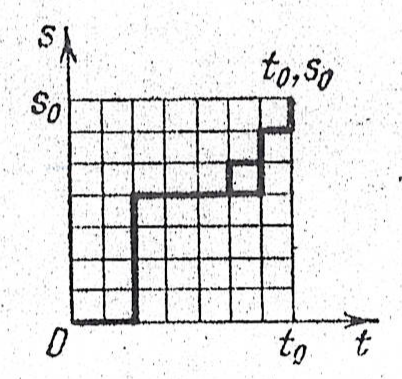
\includegraphics[scale=.24]{pic1}\hs{1pt}
198     &\\
199     \centering\scriptsize Рис. \hs{1.5pt} 170. \hs{0pt} К доказатель- & 
        \scriptsize Рис. \hs{2pt} 171. \hs{2pt} Криволинейный четырех- \\
200     \centering\scriptsize ству коммутативности & \scriptsize угольник 
        $\beta\gamma\delta\epsilon\alpha$. \\
201     \centering\scriptsize потоков. &
202 \end{tabular}
203 \vs{7pt}
204 \footnotesize \hs{.5pt} Так, например, \hs{1pt} сторонам \hs{1pt} $(0 
    \hs{.5}\leq\hs{.5} t \hs{.5}\leq\hs{.5} t_0, s \eq 0)$ и \hs{1pt} $(t 
    \eq t_0, 0 \hs{.5}\leq\hs{.5} s \hs{.5}\leq\hs{.5} s_0)$ отвечает 
    произведение \hs{1pt} $B^{s_0}A^{t_0}$, а сторонам \hs{1pt} $(t \eq 0, 
    0 \hs{.5}\leq\hs{.5} s \hs{.5}\leq\hs{.5} s_0)$ \hs{3pt} и \hs{2pt} $(s 
    \eq s_0, 0 \hs{.5}\leq\hs{.5} t \hs{.5}\leq\hs{.5} t_0)$ --- произведение 
    $A^{t_0}B^{s_0}$.
205 \vs{.5pt}
206 \footnotesize \hs{.5pt} Кроме того, мы сопоставим каждому \hs{1pt} 
    такому пути на \hs{1pt} плоскости \hs{0pt} $(t, \hs{2pt} s)$ путь 
    \hs{1pt} на \hs{1pt} монгообразии \hs{1pt} $M$, \hs{1pt} выходящий 
    \hs{.6pt} из \hs{.59pt} точти \hs{.8pt} \textit{x}, \hs{1pt} составленный
    \hs{1pt} из \hs{.2pt} траекторий \vs{-1pt} потоков \hs{1pt} $A^{t}$ 
    \hs{.8pt} и \hs{.8pt} $B^{s}$ \hs{.1pt} (рис. 171). \hs{1pt} Если 
    \hs{1pt} пути \hs{1pt} на плоскости \hs{1pt} $(t, \hs{2pt} s)$ \hs{.5pt} 
    соответствует \vs{2pt} преобразование $A^{t_1}B^{s_1} \dots A^{t_n}
    B^{s_n}$,то на монгообразии $M$ соответствующий путь \vs{-7pt} 
    заканчивается \hs{.5pt} в точке \hs{-.8pt} $A^{t_1}B^{s_1} \dots 
    A^{t_n}B^{s_n}$\textit{x}.
207 \hs{.5pt} Наша цель --- доказать, что все эти пути в действительности 
    заканчиваются в одной точке $A^{t_0}B^{s_0} \eq A^{t_0}B^{s_0}$
    \textit{x}.
208 \hs{.5pt} Разобъем отрезки $(0 \hs{.5}\leq\hs{.5} t \hs{.5}\leq\hs{.5} 
    t_0)$ и $(0 \hs{.5}\leq\hs{.5} s \hs{.5}\leq\hs{.5} s_0)$ на \hs{1pt} 
    $N$ равных частей так,\hs{1pt} что \vs{-1pt} весь \hs{1pt} прямоугольник 
    \hs{1pt} разделится на $N^2$ \hs{.5pt} маленьких прямоугольников. 
    Переход \vs{-1pt} от \hs{1pt} сторон $(0, \hs{2pt} 0)$ --- $(0, 
    \hs{2pt} t_0)$ --- $(s_0, \hs{2pt} t_0)$ к сторонам $(0, \hs{2pt} 0)$
     --- $(s_0, \hs{2pt} 0)$ --- $(s_0, \hs{2pt} t_0)$ можно \vs{-1pt}
    совершить \hs{.5pt} в \hs{1pt} $N^2$ шагов, \hs{1pt} в каждом из которых
    \hs{1pt} пара соведних сторон малень- \vs{-1pt} кого прямоугольника 
    \hs{1pt} заменяется другой парой \hs{1pt} (рис. 172).
209 \end{document}
\end{verbatim}
\end{small}

} 
\end{document}